\section{圆}
\subsection{圆的方程}
\begin{definition}
    圆\index{圆}是平面内到一定点的距离等于定长的点的集合。
\end{definition}
\begin{theorem}[圆的标准方程]\index{圆!圆的标准方程}
    \begin{equation}
        (x-a)^2+(y-b)^2=r^2
    \end{equation}
\end{theorem}

\begin{corollary}[圆与点的位置关系]
    判断一个点在圆内、圆上还是圆外的方法：设\(\odot C\)的圆心为$C(a,b)$，半径为\(r>0\)，则
    
    点$(x_0,y_0)$在\(\odot C\)内\(\Leftrightarrow   (x_0-a)^2+(y_0-b)^2>r^2\)；

    点$(x_0,y_0)$在\(\odot C\)上\(\Leftrightarrow   (x_0-a)^2+(y_0-b)^2=r^2\)；

    点$(x_0,y_0)$在\(\odot C\)外\(\Leftrightarrow   (x_0-a)^2+(y_0-b)^2<r^2\)。
\end{corollary}
\begin{example}
    已知圆\(C\)的方程为\(f(x,y)=0\)，点\(A(x_0,y_0)\)在圆外，点\(B(x',y')\)在圆上，
    则求\(f(x,y)-f(x_0,y_0)+f(x',y')=0\)表示的曲线。
\end{example}
\begin{exercise}
    观察下列方程，写出方程对应的轨迹。如果是圆，请指出圆心和半径。
    \begin{enumerate}
        \item \[(x+1)^2+(y-3)^2=2\]
        \item \[x^2+(y-4)^2=-4\]
        \item \[(x-4)^2+(y+2)^2=0\]
    \end{enumerate}
\end{exercise}

\begin{example}
    根据下列条件，求圆的标准方程：

   (1)圆心在点$C(-2,1)$，且过点$A(2,2)$；

   (2) 过点$(0,1)$和点$(2,1)$，半径为\(\sqrt{5}\)。

   (3) 设\(\odot C\)的圆心$C$在直线$l$：$2x-7y+8=0$上，$A(6,0),\ B(1,5)$都是$C$上的点。
\end{example}
\begin{theorem}[垂径定理]
    垂直于弦的直径平分弦且平分这条弦所对的两条弧；
    平分弦（非直径）的直径垂直于这条弦，并且平分这条弦所对的两条弧；
    垂直平分弦的弦一定是直径，且平分另一条弦所对的两条弧。

    实际上在一个圆中有两条弦，若其中一条弦满足下列五个条件中的两个，则必定满足其他三个条件：

    （1）平分另一条弦所对的优弧
    
    （2）平分另一条弦所对的劣弧
    
    （3）平分另一条弦
    
    （4）垂直于另一条弦
    
    （5）过圆心（或是直径）

\end{theorem}
如果将圆的标准方程展开
\begin{align*}
    (x-a)^2+(y-b)^2&=r^2\\
    x^2-2ax+a^2+y^2-2by+b^2&=r^2\\
    x^2+y^2-2ax-2by+(a^2+b^2-r^2)&=0\\
\end{align*}
得到类似这样的式子，相比配方好的标准式，它们更符合我们一般认知中的方程。
\begin{theorem}[圆的一般方程]\index{圆!圆的一般方程}
    \begin{equation}
        x^2+y^2+Dx+Ey+F=0
    \end{equation}
\end{theorem}
\begin{jie}
    \begin{align*}
        x^2+y^2+Dx+Ey+F&=0\\
        x^2+Dx+\frac{D^2}{4}+y^2+Ey+\frac{E^2}{4}&=\frac{D^2}{4}+\frac{E^2}{4}-F\\
        (x+\frac{D}{2})^2+(y+\frac{E}{2})^2&=\frac{D^2}{4}+\frac{E^2}{4}-F\\
    \end{align*}
    \[r=\frac{\sqrt{D^2+E^2-4F}}{2}\]
\end{jie}

\begin{example} 判断下列方程是否是圆的方程，如果是，写出圆的圆心坐标与平径；如果不是，说明理由。

    $(1)  x^{2}+y^{2}+4 x-6 y-12=0 $；

$(2)  4 x^{2}+4 y^{2}-8 x+4 y-15=0 $；

$(3)  x^{2}+y^{2}-6 x+10=0 $；

$(4)x^{2}+y^{2}+4x+2y+5=0$.
\end{example}
圆系

\begin{example}
    求经过\(A,B,C\)三点的圆的方程：

    \((1)A(0,0),B(2,0),C(0,2)\)

    \((2)A(5,1),B(7,-3),C(2,-8)\)
\end{example}
\begin{jie}
    \ 

    $(1)$

    \((2)\)
    \begin{way1}
        
    \end{way1}
    \begin{way2}
        设圆的方程为\((x-a)^2+(y-b)^2=r^2\)
    \end{way2}
    \begin{way3}
        设圆的方程为\(x^2+y^2+Dx+Ey+F=0\)
    \end{way3}
\end{jie}
\begin{theorem}
    二元二次方程\begin{equation}
        Ax^2+By^2+Cxy+Dx+Ey+F=0
    \end{equation}
    在平面直角坐标系中对应的曲线一定是
    圆、椭圆、双曲线、抛物线、两条（相交、平行或重合的）直线、一个点、空集之一。
\end{theorem}
\begin{theorem}
    $x^{2}+y^{2}+D_{1} x+E_{1} y+F_{1}=0$ ，$C_{2}: x^{2}+y^{2}+D_{2} x+E_{2} y+F_{2}=0$

    \begin{equation}
        \lambda(x^{2}+y^{2}+D_{1} x+E_{1} y+F_{1})+\mu(x^{2}+y^{2}+D_{2} x+E_{2} y+F_{2})=0
    \end{equation}
\end{theorem}
\clearpage
\subsection{直线、圆的位置关系}
\begin{definition}[直线与圆的位置关系]\index{圆!直线与圆的位置关系}
    如图\ref{图圆与直线相交}所示，直线与圆有两个公共点
时，称直线与圆相交，且称直线为圆的割线；
如图\ref{图圆与直线相切}所示，直线与圆只有一个公共点时，称直线与圆相切，且称直线为圆的切线，称公共点为切点；
如图\ref{图圆与直线相离}所示，直线与圆没有公共点时，称直线与圆相离。
\end{definition}
\begin{figure}[h]
    \centering
    \begin{subfigure}[b]{0.3\textwidth}
        \centering
        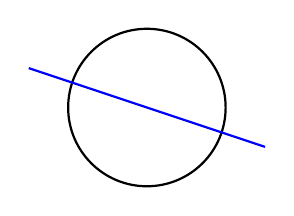
\begin{tikzpicture}
            \draw[thick, black] (0,0) circle (1cm); % 圆
            \draw[thick, blue] (-1.5,0.5) -- (1.5,-0.5); % 相交直线
        \end{tikzpicture}
        \caption{相交}
        \label{图圆与直线相交}
    \end{subfigure}
    \hfill
    \begin{subfigure}[b]{0.3\textwidth}
        \centering
        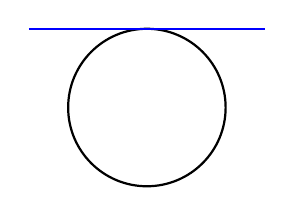
\begin{tikzpicture}
            \draw[thick, black] (0,0) circle (1cm); % 圆
            \draw[thick, blue] (-1.5,1) -- (1.5,1); % 相切直线
        \end{tikzpicture}
        \caption{相切}
        \label{图圆与直线相切}
    \end{subfigure}
    \hfill
    \begin{subfigure}[b]{0.3\textwidth}
        \centering
        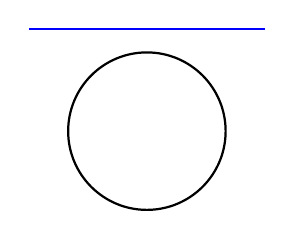
\begin{tikzpicture}
            \draw[thick, black] (0,0) circle (1cm); % 圆
            \draw[thick, blue] (-1.5,1.3) -- (1.5,1.3); % 相离直线
        \end{tikzpicture}
        \caption{相离}
        \label{图圆与直线相离}
    \end{subfigure}
    \caption{圆与直线的关系示意图}
\end{figure}

\begin{theorem}
    如果圆的的半径为\(r\)，圆心到直线的距离为\(d\)，则

    \centering     直线与圆相交\(\Leftrightarrow d<r\)；

    \centering     直线与圆相切\(\Leftrightarrow d=r\)；

    \centering     直线与圆相离\(\Leftrightarrow d>r\)。
\end{theorem}
\begin{jie}
    
\end{jie}




\begin{example}
    判断直线\(l:y=-x+5\)与圆\(C:x^2+y^2=12\)的位置关系。
\end{example}
\begin{exercise}
    
\end{exercise}
\begin{jie}
    
    \qed
\end{jie}

在这里阐释一下相切的意义。从初中到现在，一直都是使用交点个数来定义“相交”、“相切”和“相离”。
但是这个定义并不完美，在初中我们就遇到了抛物线和其对称轴的情况——直线和曲线有一个交点，却很难让人觉得这是
相切关系。在此应该用更加现代的观点重新审视“相切”这一词。







这种定义相切的方法还有很多细节要说，但是这不是这节的重点。仅仅是想解释：使用切点个数来定义相切和使用这种动态
的方法定义相切有本质的区别。
在此并没有给出一个确切的方法来计算这种动态过程产生的切线，我们将在第\ref{导数的初步认识}章
学习导数的相关知识，了解这种切线定量的计算方法。
因此暂时还是使用交点的个数来定义相切——至少在这几章内不会出现大问题。




\begin{example}根据已知条件求切线方程：

    （1）已知点\(M(1,2)\)和圆\(x^2+(y-1)^2=2\)，求在点\(M\)的圆的切线；

    （2）已知点\(N(1,1)\)和圆\((x-3)^2+(y+1)^2=4\)，求过点\(M\)的圆的切线。
\end{example}
区分“在某处的切线”和“过某处的切线”。
\begin{theorem}[切线长定理]
    从圆外一点引圆的两条切线，它们的切线长相等，且这点与圆心的连线平分两条切线的夹角。
    \begin{definition}[切线长]
        经过圆外一点做圆
        的切线，这点和切点之间的线段的长叫做这点到圆的切线长。
    \end{definition}
\end{theorem}
\begin{theorem}\label{thm:圆的切线方程定理}\index{圆!圆的切线方程}
    圆\(x^2+y^2=r^2\)在点\((x_0,y_0)\)处的切线方程为
    \begin{equation}\label{equ:圆的切线方程}
        x_0x+y_0y=r^2
    \end{equation}
\end{theorem}
\begin{corollary}\label{cor:圆的切线方程推论}
    \ 

    圆\((x-a)^2+(y-b)^2=r^2\)在点\((x_1,y_1)\)处的切线方程为
    \begin{equation}
        (x_1-a)(x-a)+(y_1-b)(y-b)=r^2
    \end{equation}

    圆\(x^2+y^2+Dx+Ey+F=0\)在点\((x_2,y_2)\)处的切线方程为
    \begin{equation}
        x_2x+y_2y+D\frac{x_2+x}{2}+E\frac{y_2+y}{2}+F=0
    \end{equation}
\end{corollary}
定理\ref{thm:圆的切线方程定理}、推论\ref{cor:圆的切线方程推论}给了一个极强的条件——知道了曲线上的点，可以直接写出在这一点
的切线方程。那如果这个点不在曲线上，方程\ref{equ:圆的切线方程}有什么含义呢？

\begin{theorem}
    若点\(x_0,y_0\)在圆\(x^2+y^2=r^2\)外，则方程\[x_0x+y_0y=r^2\]表示切点弦所在直线的方程。
\end{theorem}









\begin{example}
    已知圆\(C:x^2+y^2+Dx+Ey+F=0\)和点\(M(x_0,y_0)\)为圆外一点，求\(M\)到圆\(C\)的切线长。
\end{example}
\begin{jie}
    \[(x_0+\frac{D}{2})^2+(y_0+\frac{E}{2})^2=l^2+\frac{D^2}{4}+\frac{E^2}{4}-F\]

\qed
\end{jie}

\begin{example}
    已知直线 $ l: x+y+2=0  $与圆$  C: x^{2}+y^{2}=9$  相交于 $ A, B$  两点.

    （1）求线段 $ A B $ 的长；

    （2） 求线段  $A B $ 中点的坐标。
\end{example}

\begin{example}
    若  $P(x, y) $ 是圆 $ C:(x-3)^{2}+y^{2}=1  $上的任意一点, 求 $ P(x, y) $ 到直线 $ x-y+1=0 $ 的距离的最大值和最小值。
\end{example}

\begin{definition}
    
\end{definition}
\begin{theorem}
xxxxx
\vspace*{-0.3cm}
    \begin{align*}
        \text{两个圆外离} & \Leftrightarrow d > r_{1} + r_{2} \\
        \text{两个圆外切} & \Leftrightarrow d = r_{1} + r_{2} \\
        \text{两个圆相交} & \Leftrightarrow \left| r_{1} - r_{2} \right| < d < r_{1} + r_{2} \\
        \text{两个圆内切} & \Leftrightarrow d = \left| r_{1} - r_{2} \right| \\
        \text{两个圆内含} & \Leftrightarrow d < \left| r_{1} - r_{2} \right| \\
    \end{align*}
    \vspace*{-1.4cm}
\end{theorem}
\begin{exercise}
    分别指出下列两圆的位置关系 (外离、外切、相交、内切、内含):

(1) $ x^{2}+y^{2}-4 x-6 y+9=0 \text{和}   x^{2}+y^{2}+12 x+6 y-19=0 ;$

(2) $ x^{2}+y^{2}+2 x-2 y-2=0 \text{和}  x^{2}+y^{2}-4 x-6 y-3=0 .$
\end{exercise}

\begin{theorem}
    若两圆  $C_{1}: x^{2}+y^{2}+D_{1} x+E_{1} y+F_{1}=0, C_{2}: x^{2}+y^{2}+D_{2} x+E_{2} y+F_{2}=0  $
    相交于 $ A, B  $两点，则直线 $ A B  $的方程为 
    \begin{equation}\label{equ:根轴方程}
         \left(D_{1}-D_{2}\right) x+\left(E_{1}-E_{2}\right) y+F_{1}-F_{2}=0 
    \end{equation}

    若两圆相切，则方程\ref{equ:根轴方程}是经过两圆切点的公切线；

    \begin{definition}[根轴]\index{圆!根轴}
        在平面上任给两不同心的圆，则到两圆切线长相等的点的集合是一条直线，这条线称为这两个圆的根轴。
    \end{definition}

    方程\ref{equ:根轴方程}（在有意义的情况下）总是两圆的根轴。
\end{theorem}
\begin{exercise}
     若圆 $x^{2}+y^{2}=1 $ 与 $ x^{2}+y^{2}+2 x-2 y=0 $ 相交于$  A ,B $ 两点，求直线  $A B $的方程。
\end{exercise}

接下来研究一下两个圆公切线的数量及求法。

\begin{theorem}[切线的数量]
\ 

    \begin{center}
        \begin{minipage}{0.3\textwidth} % 设置 minipage 的宽度，例如 50% 的文本宽度
          \raggedright % 使文本左对齐
          两个圆外离：四条切线

       两个圆外切：三条切线

       两个圆相交：两条切线

       两个圆内切：一条切线

      两个圆内含：零条切线
        \end{minipage}
      \end{center}
\end{theorem}

\begin{example}
 求圆 $C_1:x^{2}+y^{2}=1 $和$C_2:(x-3)^{2}+(y-4)^{2}=16 $的公切线方程。
\end{example}



\clearpage

%\subsubsection{Apollonius圆}


\clearpage
\review
\clearpage
\hw
\begin{homework}
    若 $ P(x, y) $ 是圆 $ C:(x-1)^{2}+y^{2}=\dfrac{1}{4}$  上的任意一点, 求 $ P(x, y) $ 到原点的距离的最大值和最小值.
\end{homework}
\begin{homework}
    求圆  $x^{2}+y^{2}+2 x-2 a y-4=0(a \in \mathbb{R})$  的半径的最小值.
\end{homework}
\begin{homework}
    
\end{homework}
\begin{homework}
    
\end{homework}
\begin{homework}
    
\end{homework}
\begin{homework}
    
\end{homework}
\begin{homework}
    
\end{homework}
\begin{homework}
    
\end{homework}
\begin{homework}
    
\end{homework}
\clearpage
